	\begin{figure}[tbp]
		\begin{subfigure}[c]{.48\linewidth}
			\centering
			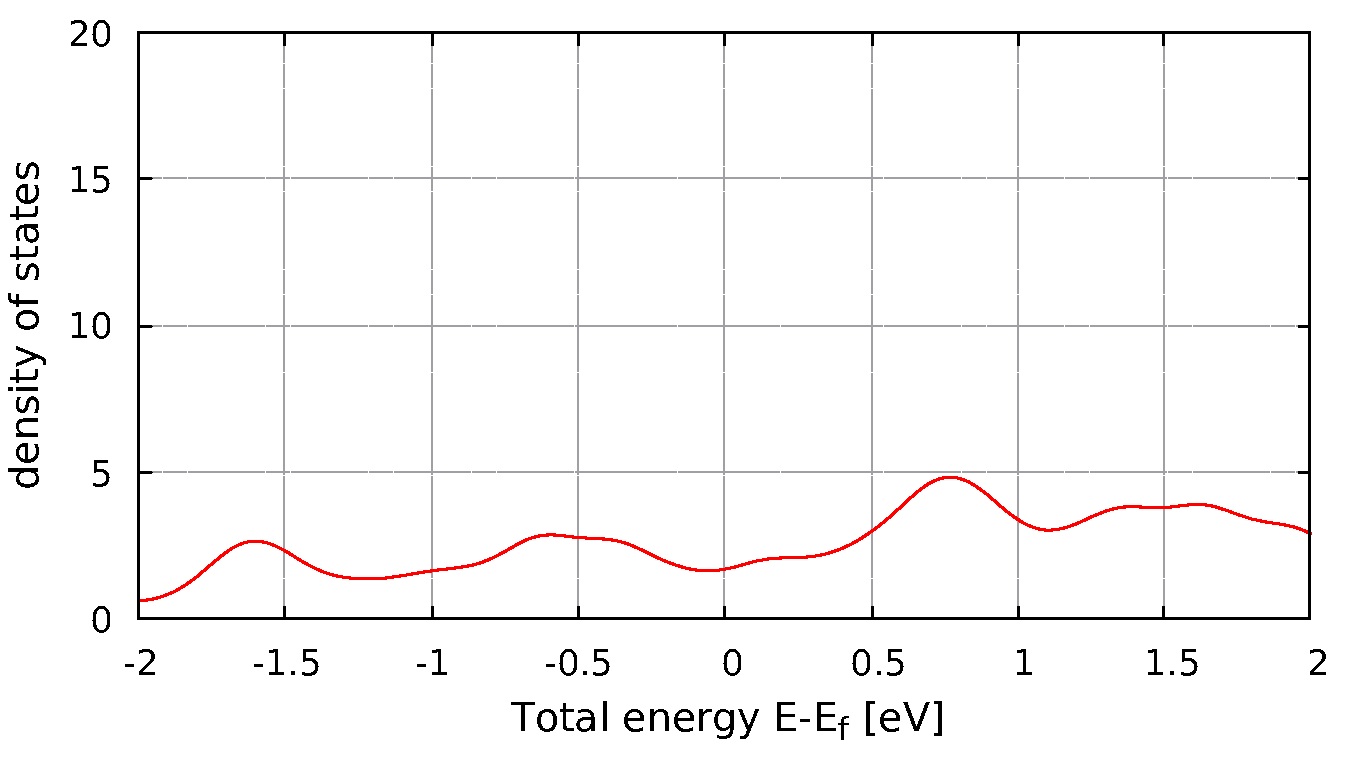
\includegraphics[width=\linewidth]{Te_and_Hg_termination/no_H_DOS_4_layers_-2_2.pdf}
			\caption{4 layers without hydrogens}
		\end{subfigure}
		\hfill
		\begin{subfigure}[c]{.48\linewidth}
			\centering
			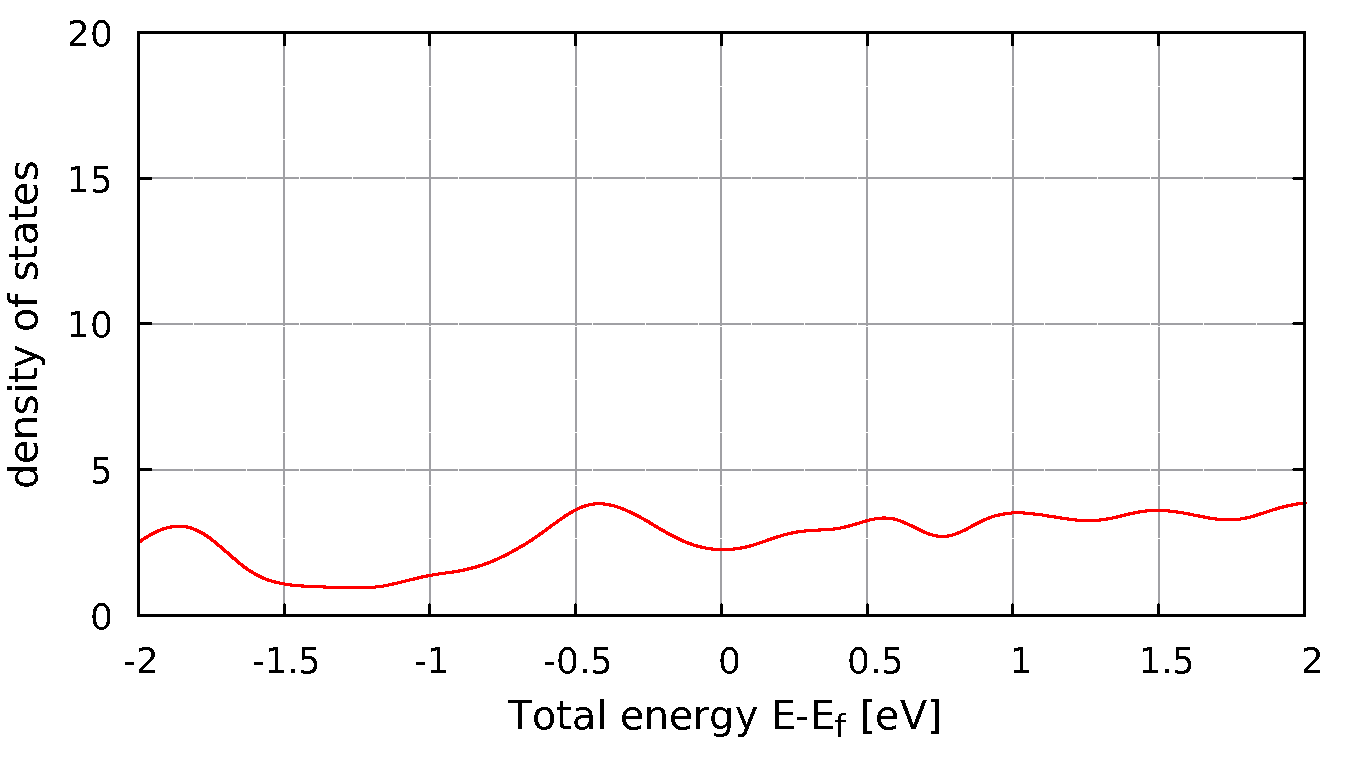
\includegraphics[width=\linewidth]{Te_and_Hg_termination/DOS_4_layers_-2_2.pdf}
			\caption{4 layers with hydrogens on the bottom}
		\end{subfigure}
		\begin{subfigure}[c]{.48\linewidth}
			\centering
			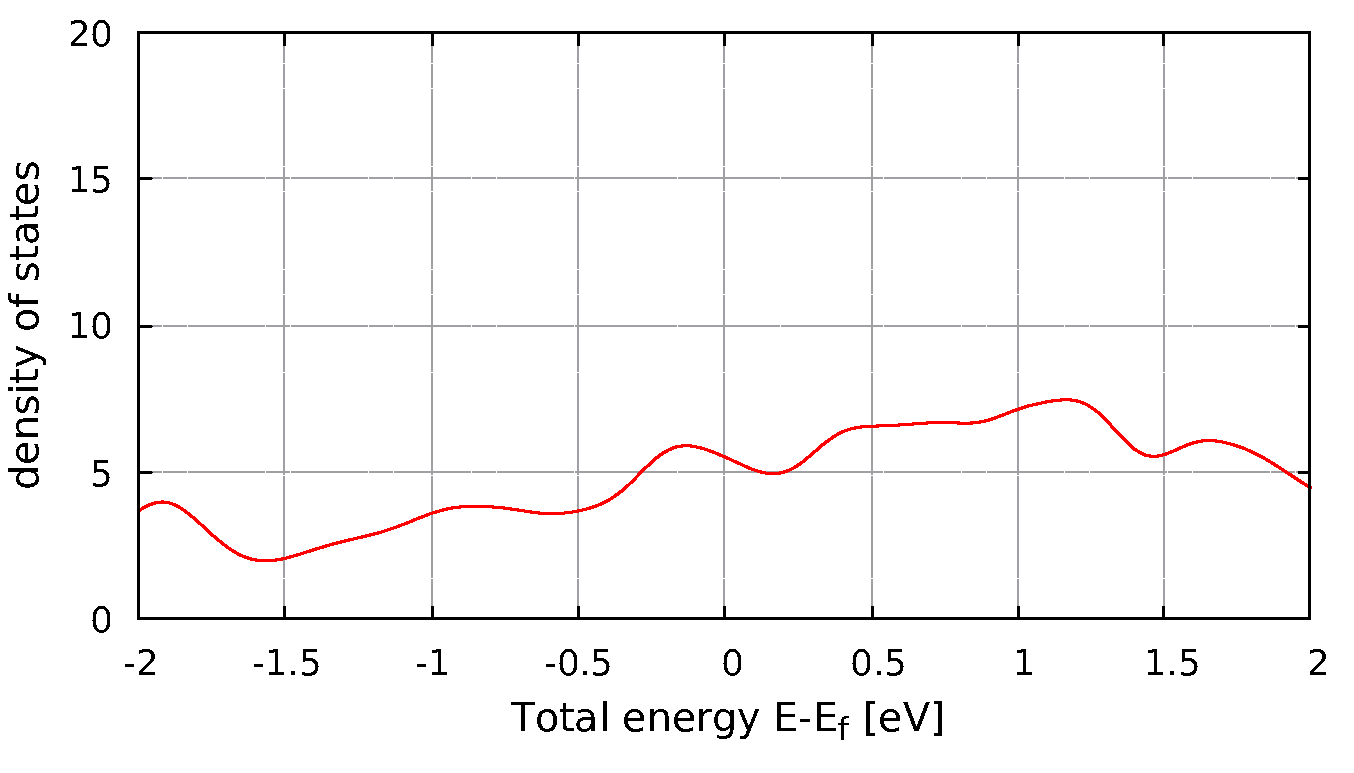
\includegraphics[width=\linewidth]{Te_and_Hg_termination/no_H_DOS_8_layers_-2_2.pdf}
			\caption{8 layers without hydrogens}
		\end{subfigure}
		\hfill
		\begin{subfigure}[c]{.48\linewidth}
			\centering
			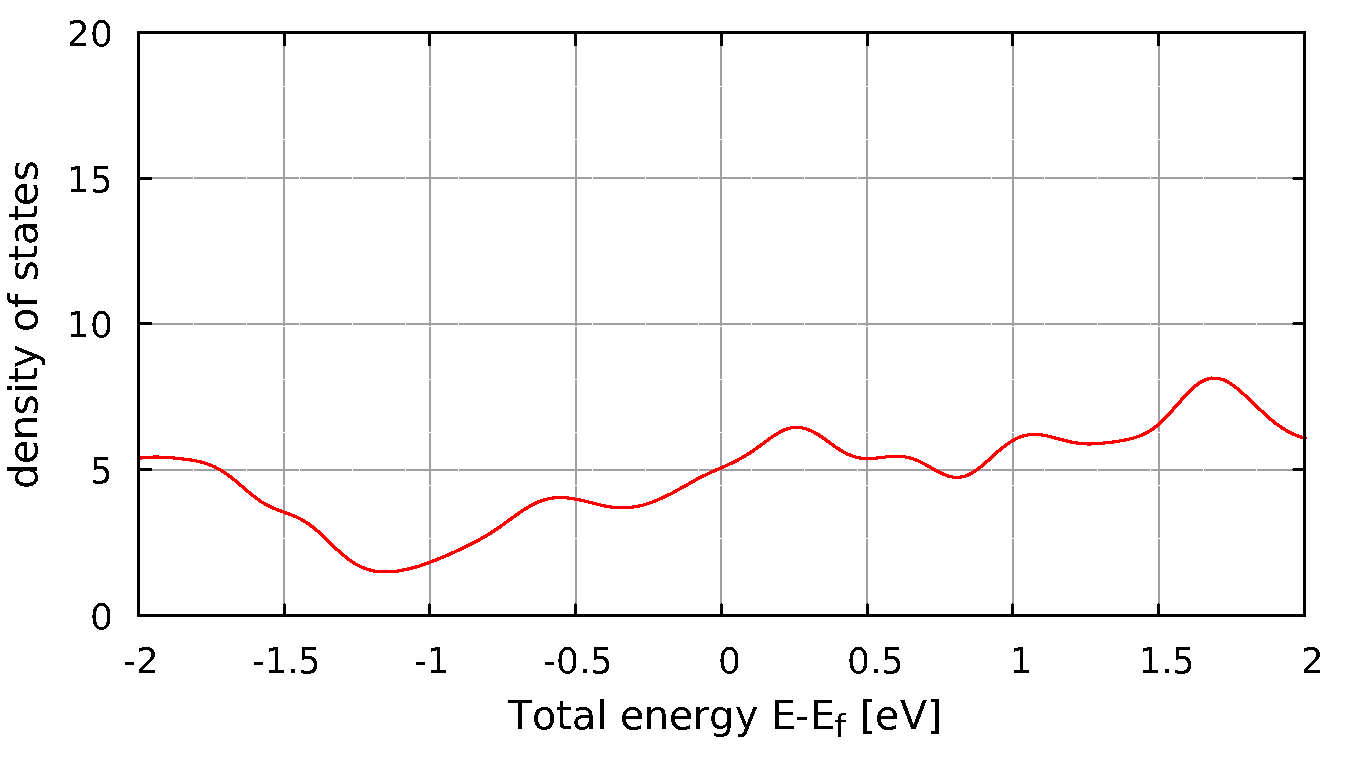
\includegraphics[width=\linewidth]{Te_and_Hg_termination/DOS_8_layers_-2_2.pdf}
			\caption{8 layers with hydrogens on the bottom}
		\end{subfigure}
		\begin{subfigure}[c]{.48\linewidth}
			\centering 
			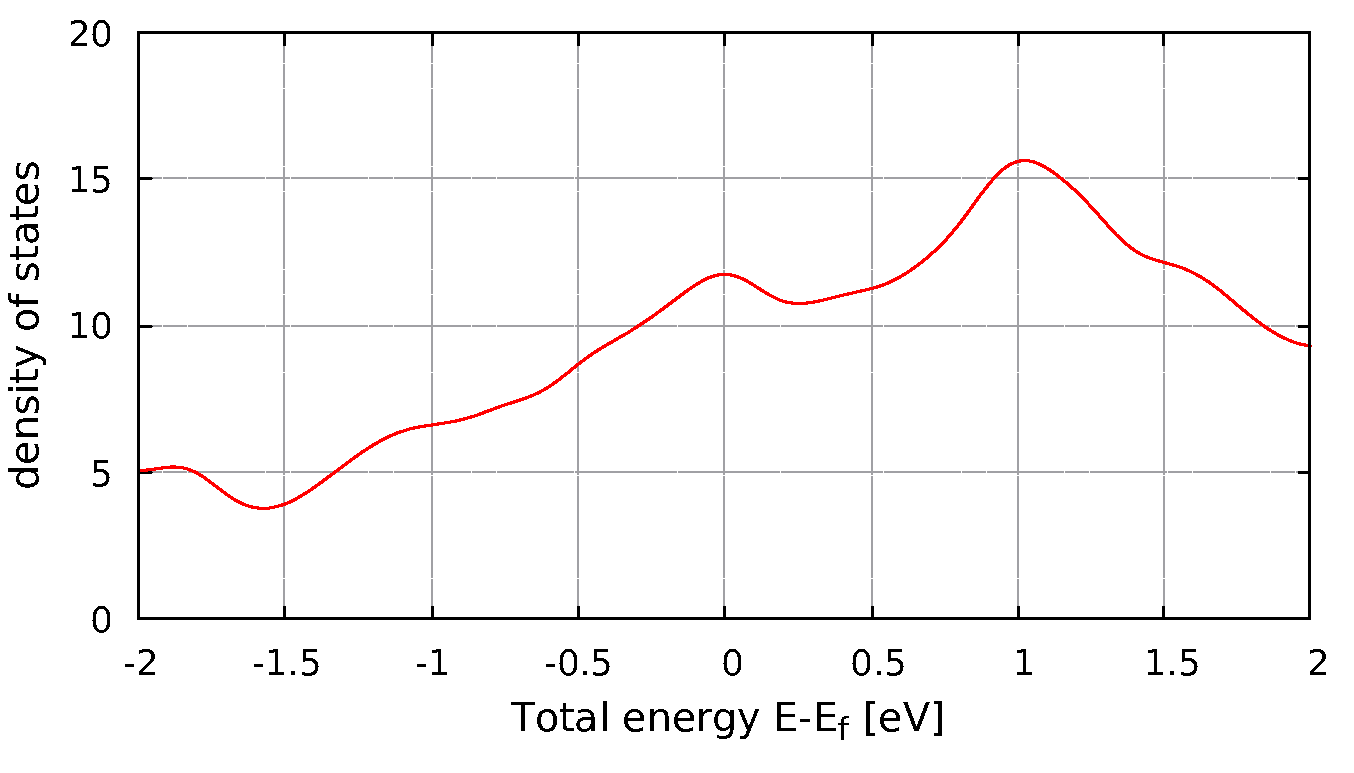
\includegraphics[width=\linewidth]{Te_and_Hg_termination/no_H_DOS_16_layers_-2_2.pdf}
			\caption{16 layers without hydrogens} \label{}
		\end{subfigure}
		\hfill
		\begin{subfigure}[c]{.48\linewidth}
			\centering
			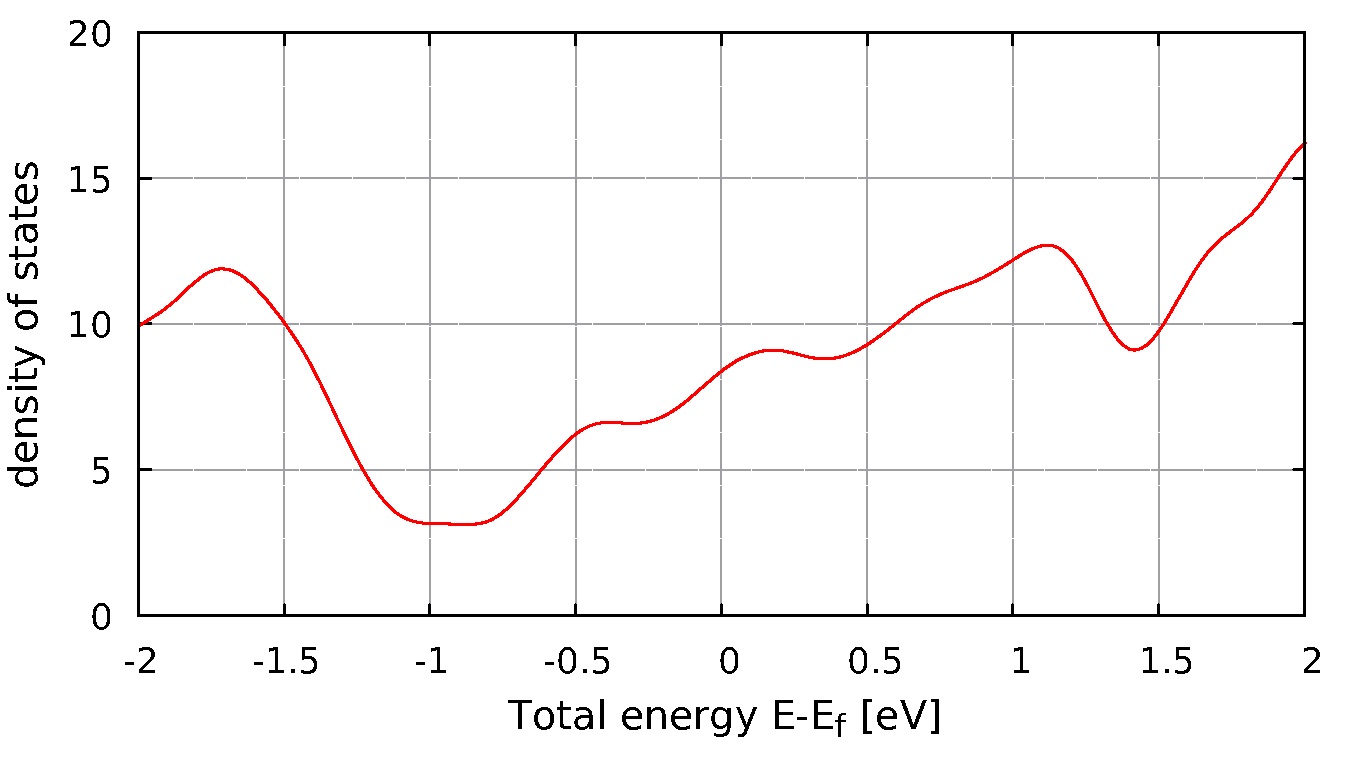
\includegraphics[width=\linewidth]{Te_and_Hg_termination/DOS_16_layers_-2_2.pdf}
			\caption{16 layers with hydrogens on the bottom}
		\end{subfigure}
		\caption{DOS of the surfaces with Te-Hg termination} 
		\label{dos_surface_even_layers}
	\end{figure}

	\begin{figure}[tbp]
		\begin{subfigure}[c]{.48\linewidth}
			\centering
			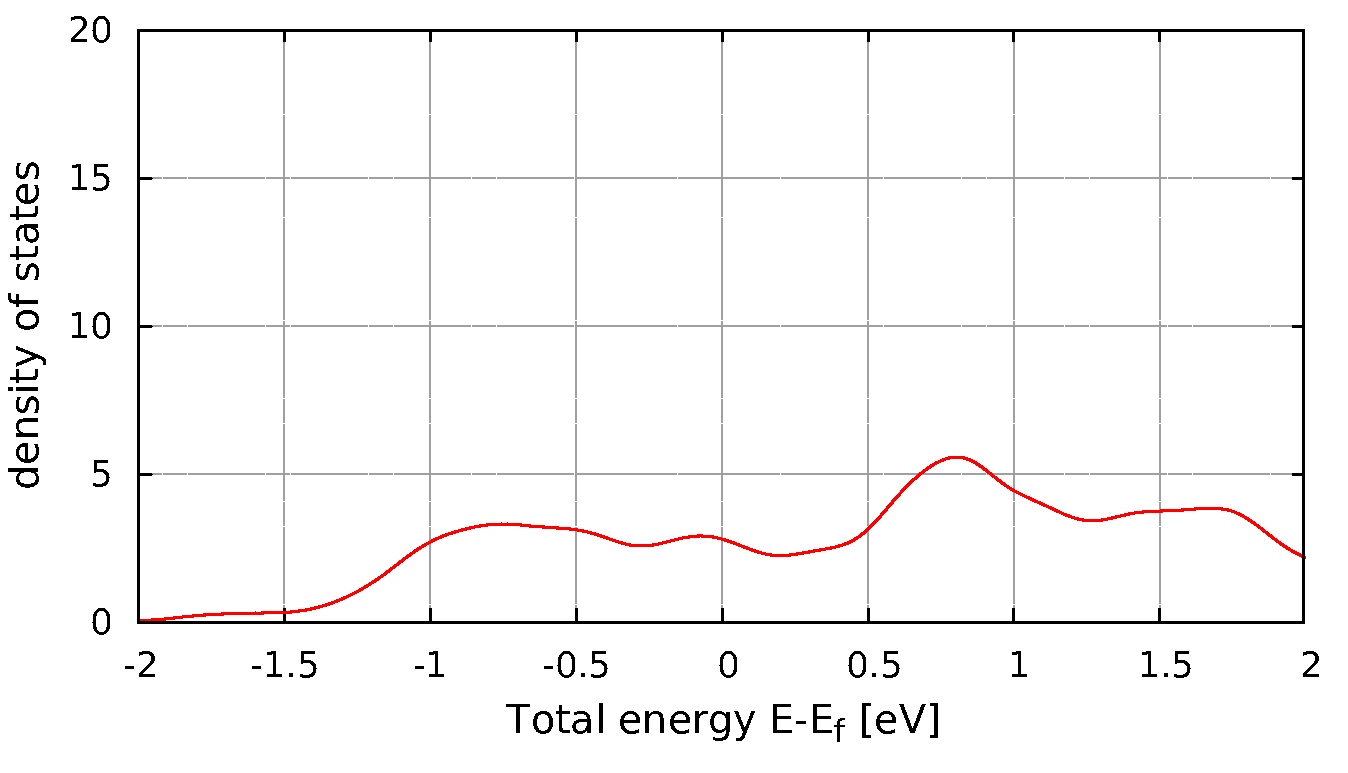
\includegraphics[width=\linewidth]{Te_termination/no_H_DOS_5_layers_-2_2.pdf}
			\caption{5 layers without hydrogens}
		\end{subfigure}
		\hfill
		\begin{subfigure}[c]{.48\linewidth}
			\centering
			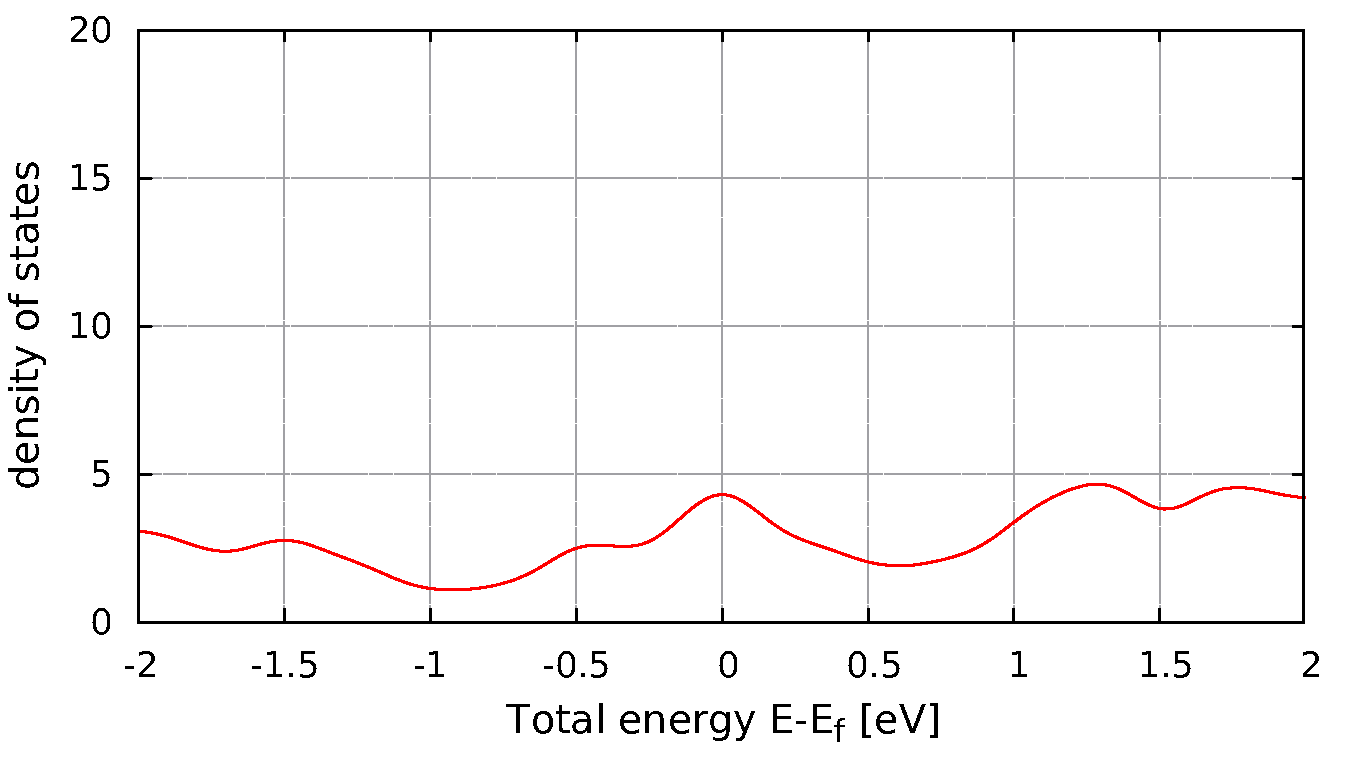
\includegraphics[width=\linewidth]{Te_termination/DOS_5_layers_-2_2.pdf}
			\caption{5 layers with hydrogens on the bottom}
		\end{subfigure}
		\begin{subfigure}[c]{.48\linewidth}
			\centering
			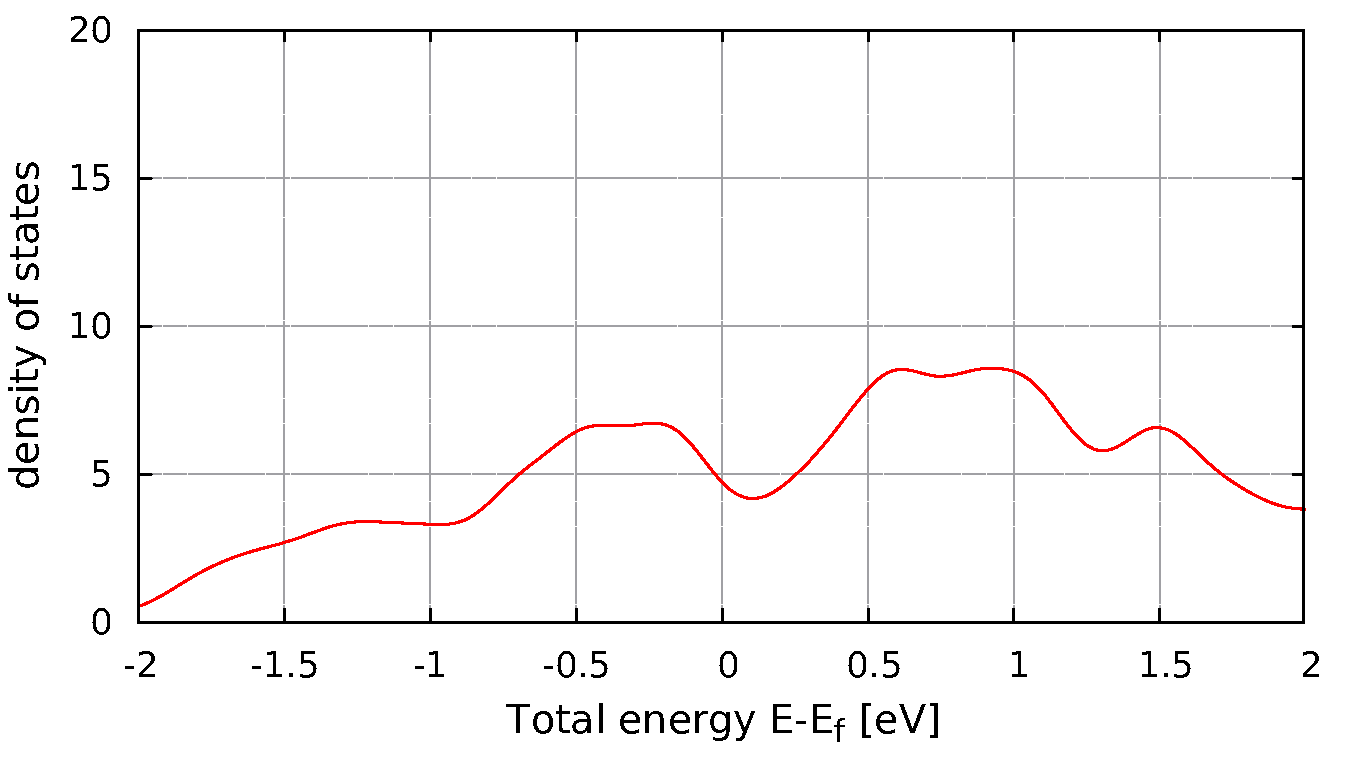
\includegraphics[width=\linewidth]{Te_termination/no_H_DOS_9_layers_-2_2.pdf}
			\caption{9 layers without hydrogens}
		\end{subfigure}
		\hfill
		\begin{subfigure}[c]{.48\linewidth}
			\centering
			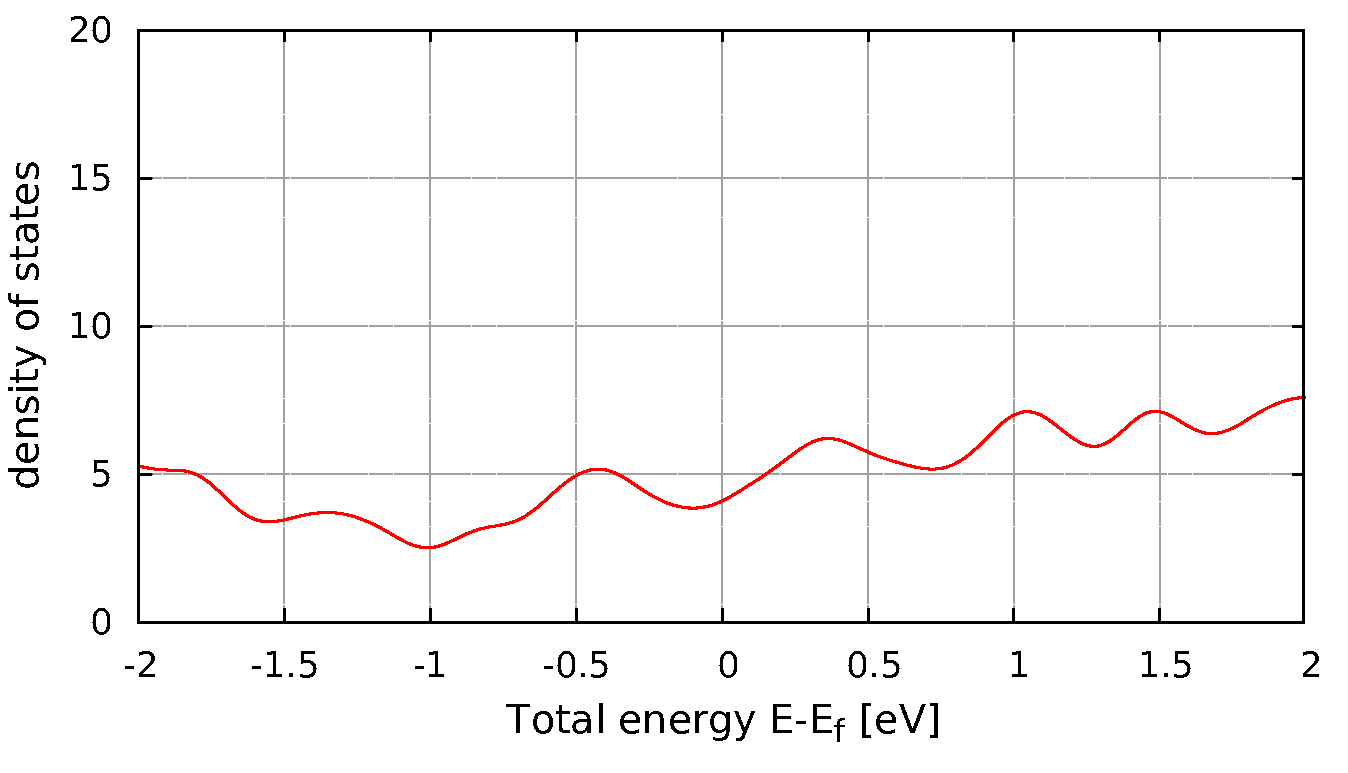
\includegraphics[width=\linewidth]{Te_termination/DOS_9_layers_-2_2.pdf}
			\caption{9 layers with hydrogens on the bottom}
		\end{subfigure}
		\begin{subfigure}[c]{.48\linewidth}
			\centering 
			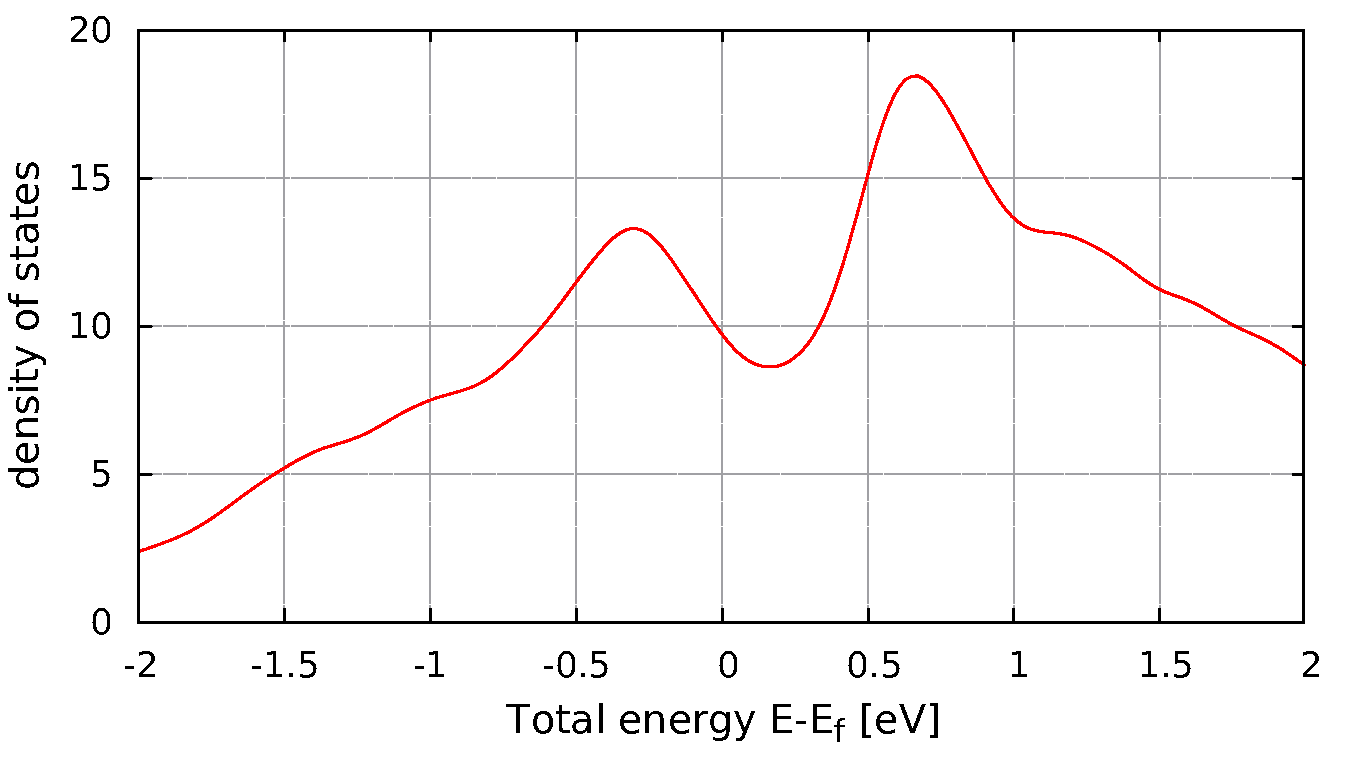
\includegraphics[width=\linewidth]{Te_termination/no_H_DOS_17_layers_-2_2.pdf}
			\caption{17 layers without hydrogens} \label{}
		\end{subfigure}
		\hfill
		\begin{subfigure}[c]{.48\linewidth}
			\centering
			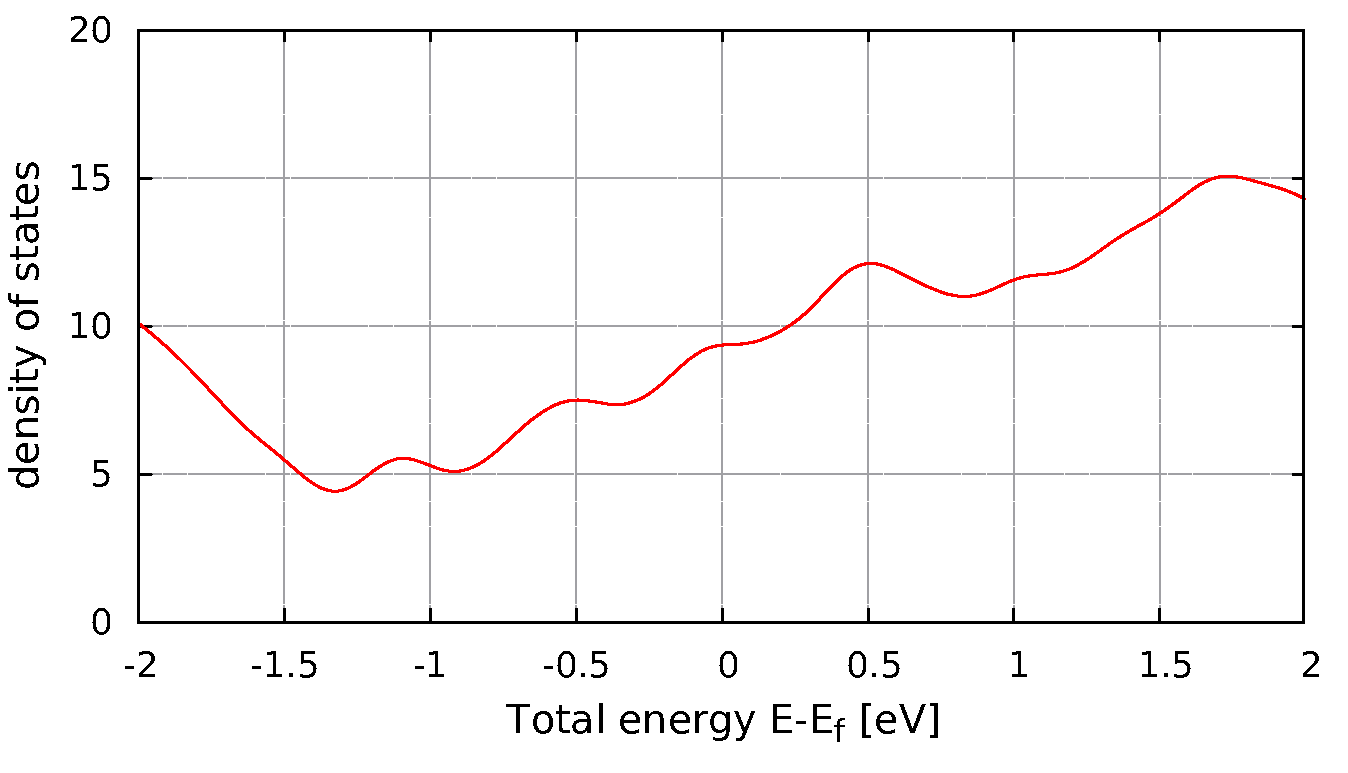
\includegraphics[width=\linewidth]{Te_termination/DOS_17_layers_-2_2.pdf}
			\caption{17 layers with hydrogens on the bottom}
		\end{subfigure}
		\caption{DOS of the surfaces with Te termination} 
		\label{dos_surface_odd_layers_Te}
	\end{figure}
	
	\begin{figure}[tbp]
		\begin{subfigure}[c]{.48\linewidth}
			\centering
			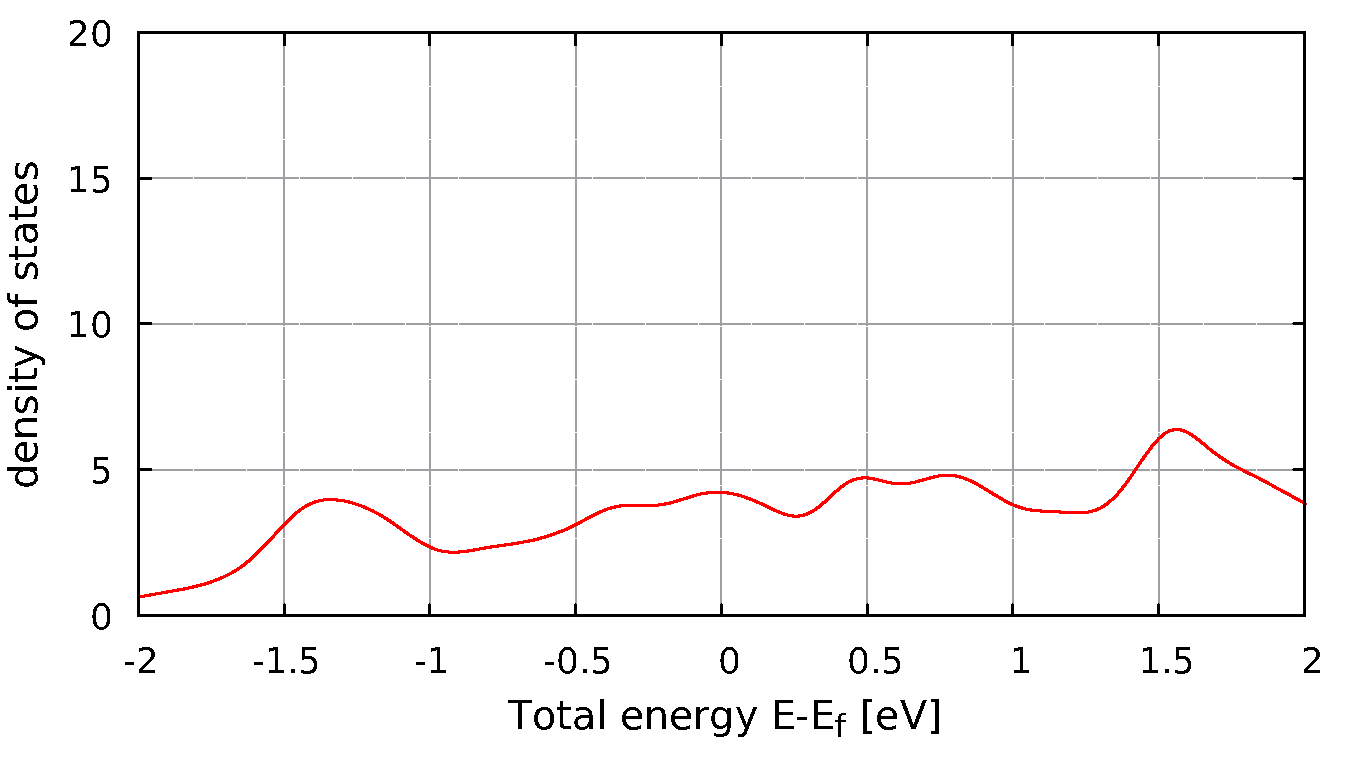
\includegraphics[width=\linewidth]{Hg_termination/no_H_DOS_5_layers_-2_2.pdf}
			\caption{5 layers without hydrogens}
		\end{subfigure}
		\hfill
		\begin{subfigure}[c]{.48\linewidth}
			\centering
			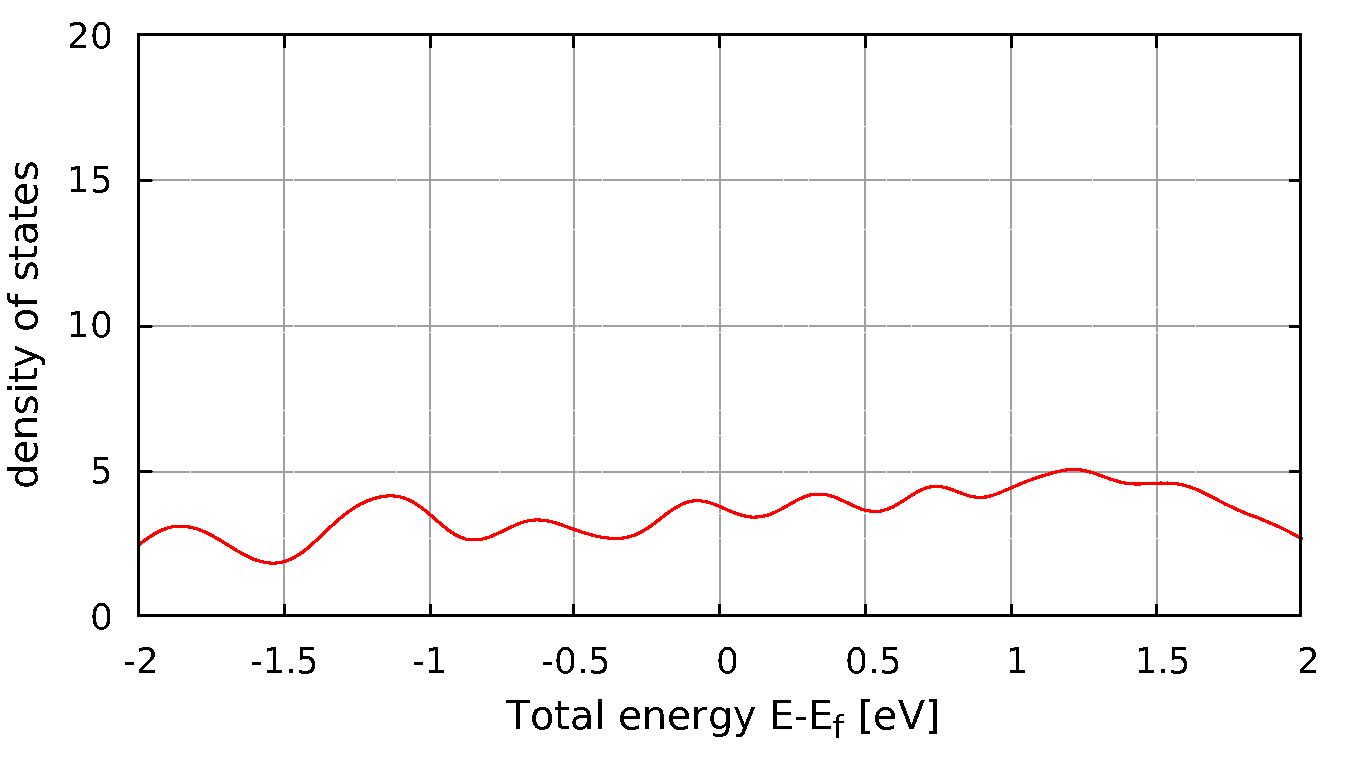
\includegraphics[width=\linewidth]{Hg_termination/DOS_5_layers_-2_2.pdf}
			\caption{5 layers with hydrogens on the bottom}
		\end{subfigure}
		\begin{subfigure}[c]{.48\linewidth}
			\centering
			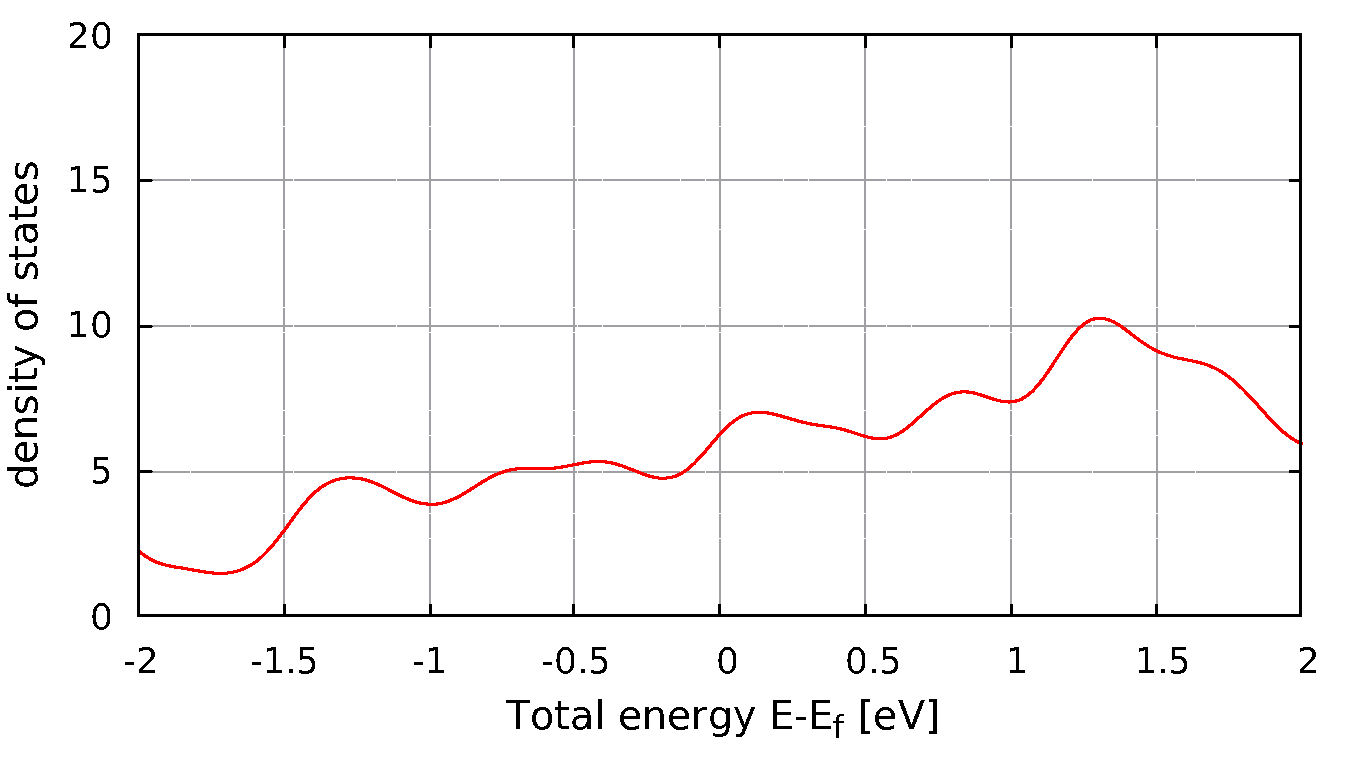
\includegraphics[width=\linewidth]{Hg_termination/no_H_DOS_9_layers_-2_2.pdf}
			\caption{9 layers without hydrogens}
		\end{subfigure}
		\hfill
		\begin{subfigure}[c]{.48\linewidth}
			\centering
			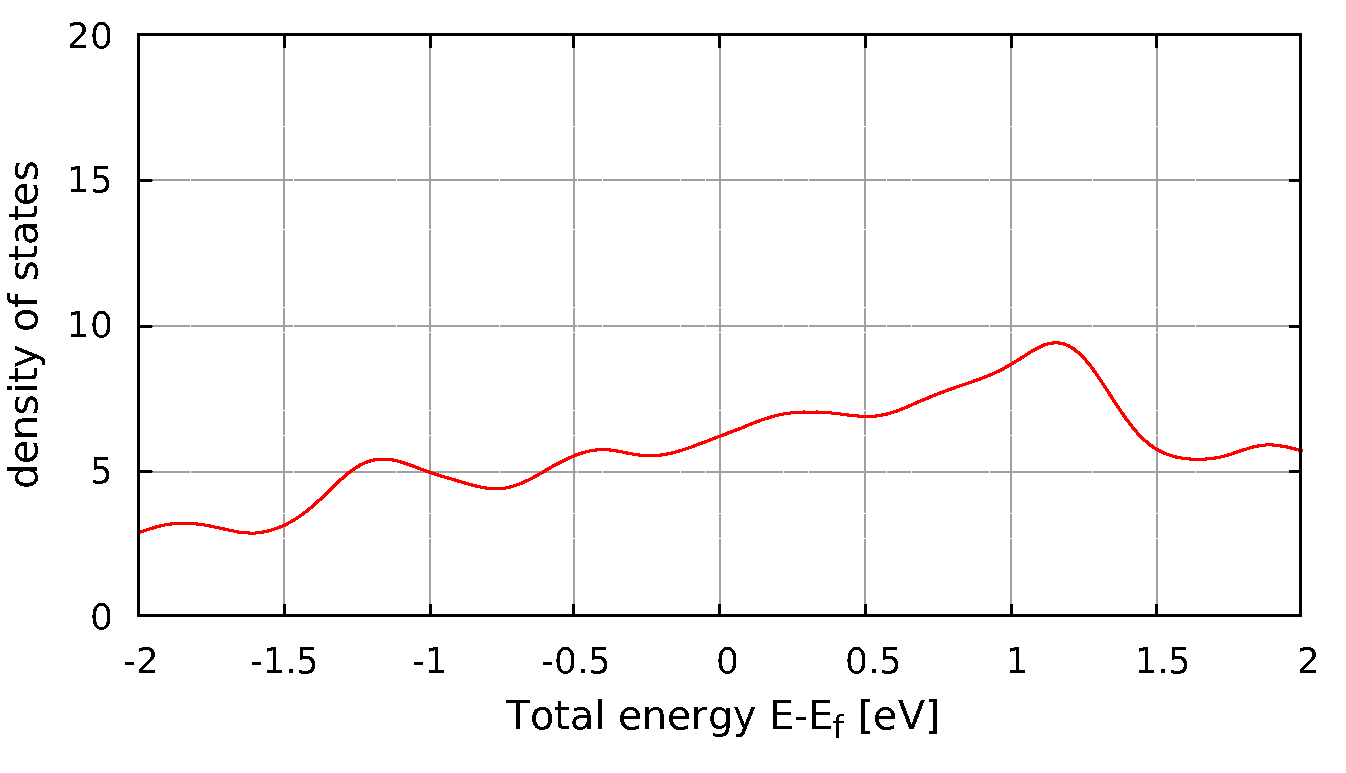
\includegraphics[width=\linewidth]{Hg_termination/DOS_9_layers_-2_2.pdf}
			\caption{9 layers with hydrogens on the bottom}
		\end{subfigure}
		\begin{subfigure}[c]{.48\linewidth}
			\centering 
			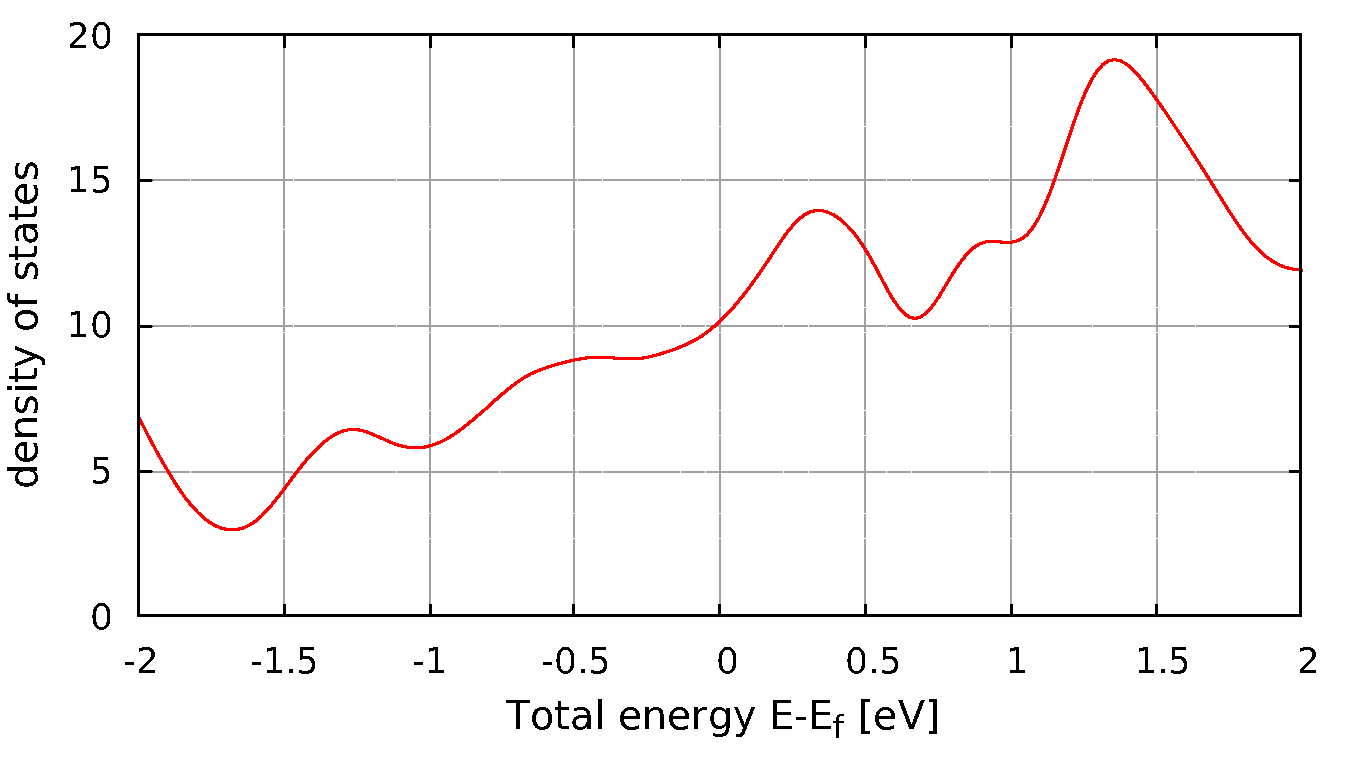
\includegraphics[width=\linewidth]{Hg_termination/no_H_DOS_17_layers_-2_2.pdf}
			\caption{17 layers without hydrogens} \label{}
		\end{subfigure}
		\hfill
		\begin{subfigure}[c]{.48\linewidth}
			\centering
			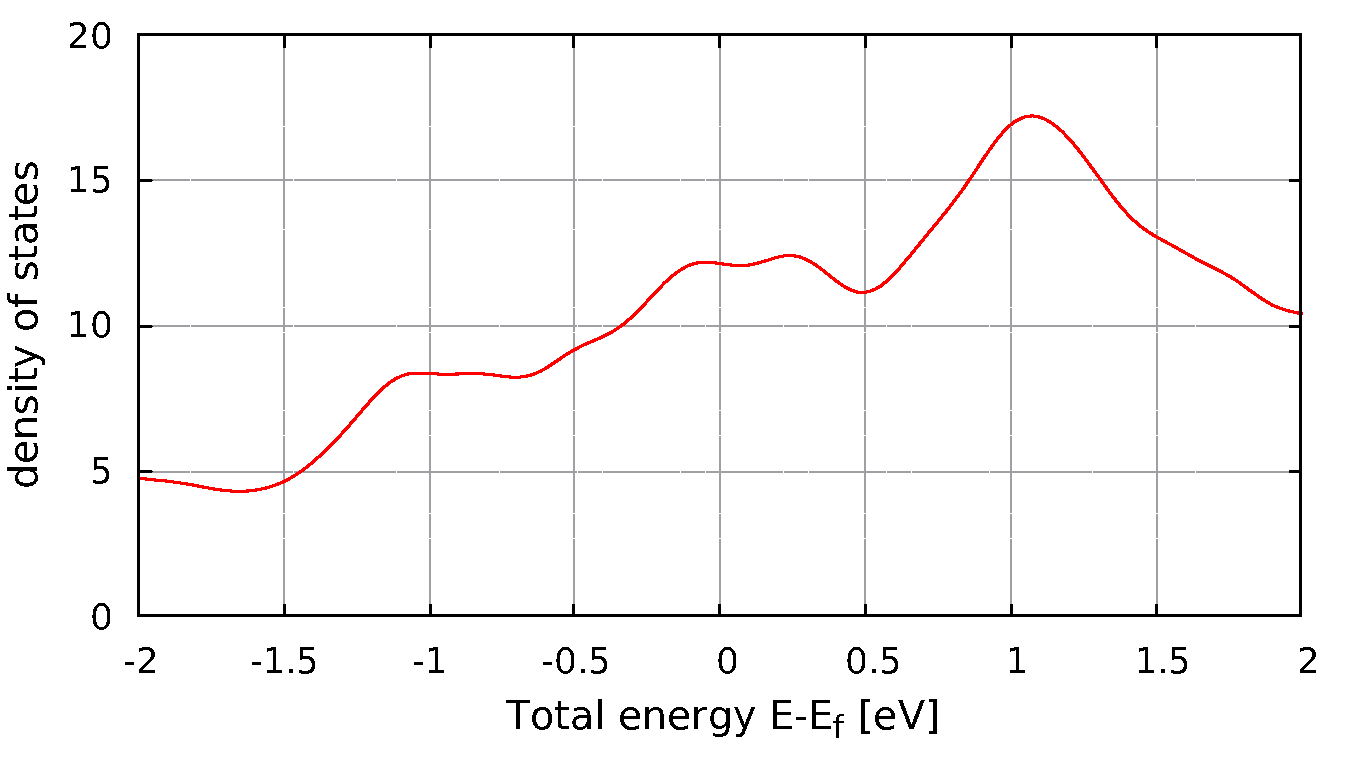
\includegraphics[width=\linewidth]{Hg_termination/DOS_17_layers_-2_2.pdf}
			\caption{17 layers with hydrogens on the bottom}
		\end{subfigure}
		\caption{DOS of the surfaces with Hg termination} 
		\label{dos_surface_odd_layers_Hg}
	\end{figure}
	The density of states (DOS) gives the number of states per interval of energy of a system which can be occupied in respect to specific energy levels \cite{tutorial2}.
	It gives no information about the actual occupation of states, but their availability. The higher the DOS at a specific energy, the more states are available there to be occupied. If the DOS is zero, there are no states able to be occupied. 
	
	In mathematical language: 
	By integrating over the energy $\epsilon$ within a unit volume cell in a small intervall $]\epsilon_0 - \Delta \epsilon , \epsilon_0 + \Delta \epsilon[$ and a certain function $g(\epsilon)$ which is called the density of states, the number of states are evaluated:
	\begin{align}
		n = \int_{\epsilon_0 - \Delta \epsilon}^{\epsilon_0 + \Delta \epsilon} \diff \epsilon g(\epsilon)
	\end{align}
	The density of states for free atoms or isolated molecules consists of dicrete energy levels, meaning it can be described by a delta function
	\begin{align}
		g(\epsilon) = \sum_i \delta(\epsilon_i - \epsilon)
	\end{align}
	For a periodic system the dos is k dependent which means, the integration of k must include the first Brillouin zone and must be averaged (divided by the volume)
	\begin{align}
		g(\epsilon) = \frac{1}{V_{BZ}} \sum_i \int_{BZ} \diff^3 k \delta (\epsilon_i(k) - \epsilon)  
	\end{align}
	But this equation is just brings exact results only for infinite k points. Since this is impossible to simulate by an numeric calculation, the infinite grid is replaced by a broadening of the delta distribution, concretely the Gaussion function with a factor $\sigma$:
	\begin{align}
		g(\epsilon) = \frac{1}{\sqrt{2\pi} \sigma} \frac{1}{n(k)} 
		\sum_i \sum_k \exp 
		\left[
			-\frac{1}{2} \left(
				\frac{\epsilon - \epsilon_i(k)}{\sigma}
			\right)^2
		\right]
	\end{align}
	The input command for FHI-aims must be set in the control.in by
	\begin{verbatim}
		# output DOS
		output dos -2. 2. 200 0.1
	\end{verbatim}
	where the first two numbers are the boundary values for the energy, the lower one first, the third is the number of energy value points taken for the integration, and the last one is the Gaussian broadening $\sigma$. 
	 
	The figures \ref{dos_surface_even_layers}, \ref{dos_surface_odd_layers_Te} and \ref{dos_surface_odd_layers_Hg} show the plots of the DOS calculations for every band structure plot that was done before. Note that the energy is now at the x axes and that the density of states the y axes in arbitrary units.   
	
%%% Local Variables:
%%% mode: latex
%%% TeX-master: "main_BA2.0"
%%% End: